\section*{Függelék}
\label{sec:fuggelek}

\begin{thebibliography}{1}
	
	\bibitem{SAW} \textbf{SF2446E} \url{https://www.rfmi.co/pdf/Datasheet/sf2446e.pdf}
	
	\bibitem{PGA} \textbf{PGA-103+} \url{https://www.minicircuits.com/pdfs/PGA-103+.pdf}
	
	\bibitem{PGA_comp} \textbf{PGA-103+ kompenzáló hálózat} \url{https://www.minicircuits.com/app/AN60-064.pdf}


\end{thebibliography}

\listoffigures

\newpage

\subsection*{Mérési eredmények}

\begin{figure}[!ht]
	\centering
	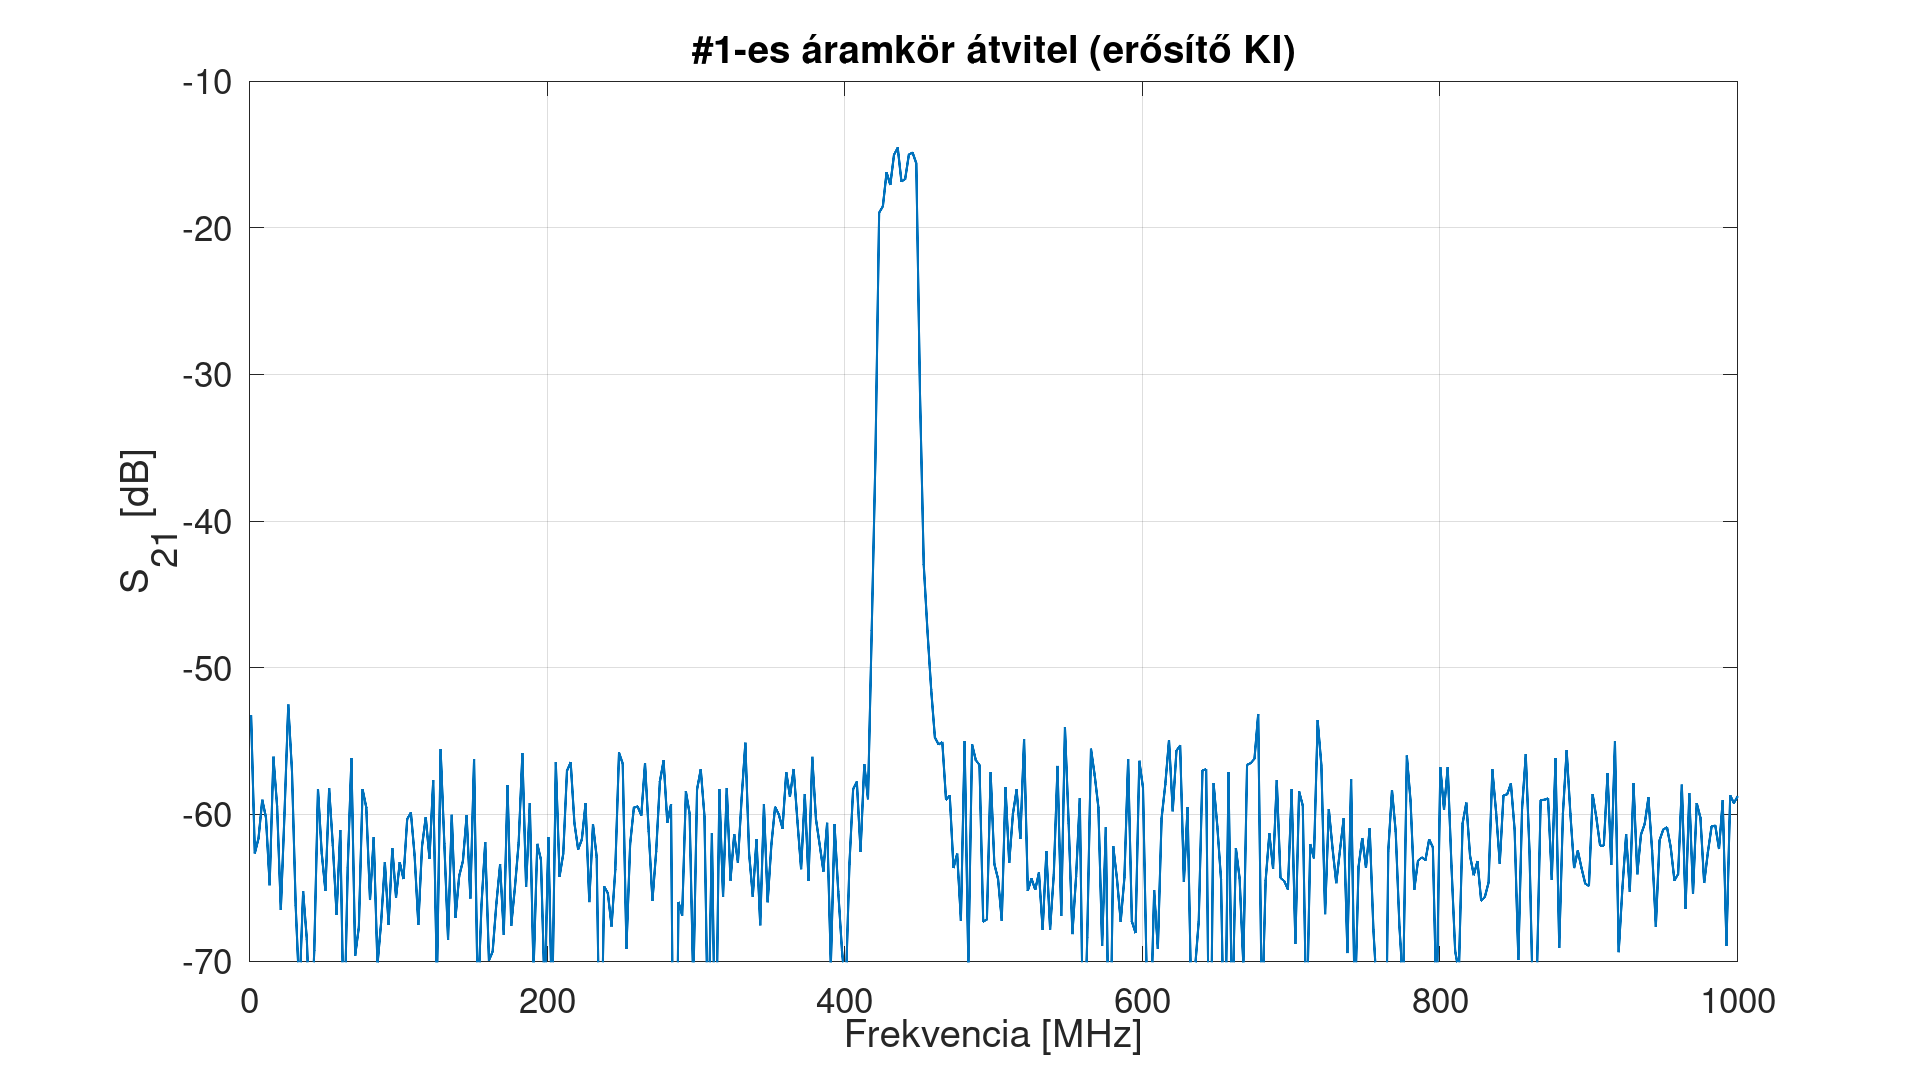
\includegraphics[keepaspectratio, width=\textwidth]{aramkor1_1.png}
	\caption{\#1-es erősítő 1\,MHz - 1\,GHz, erősítő KI}
	\label{fig:meres1}
\end{figure}

\begin{figure}[!ht]
	\centering
	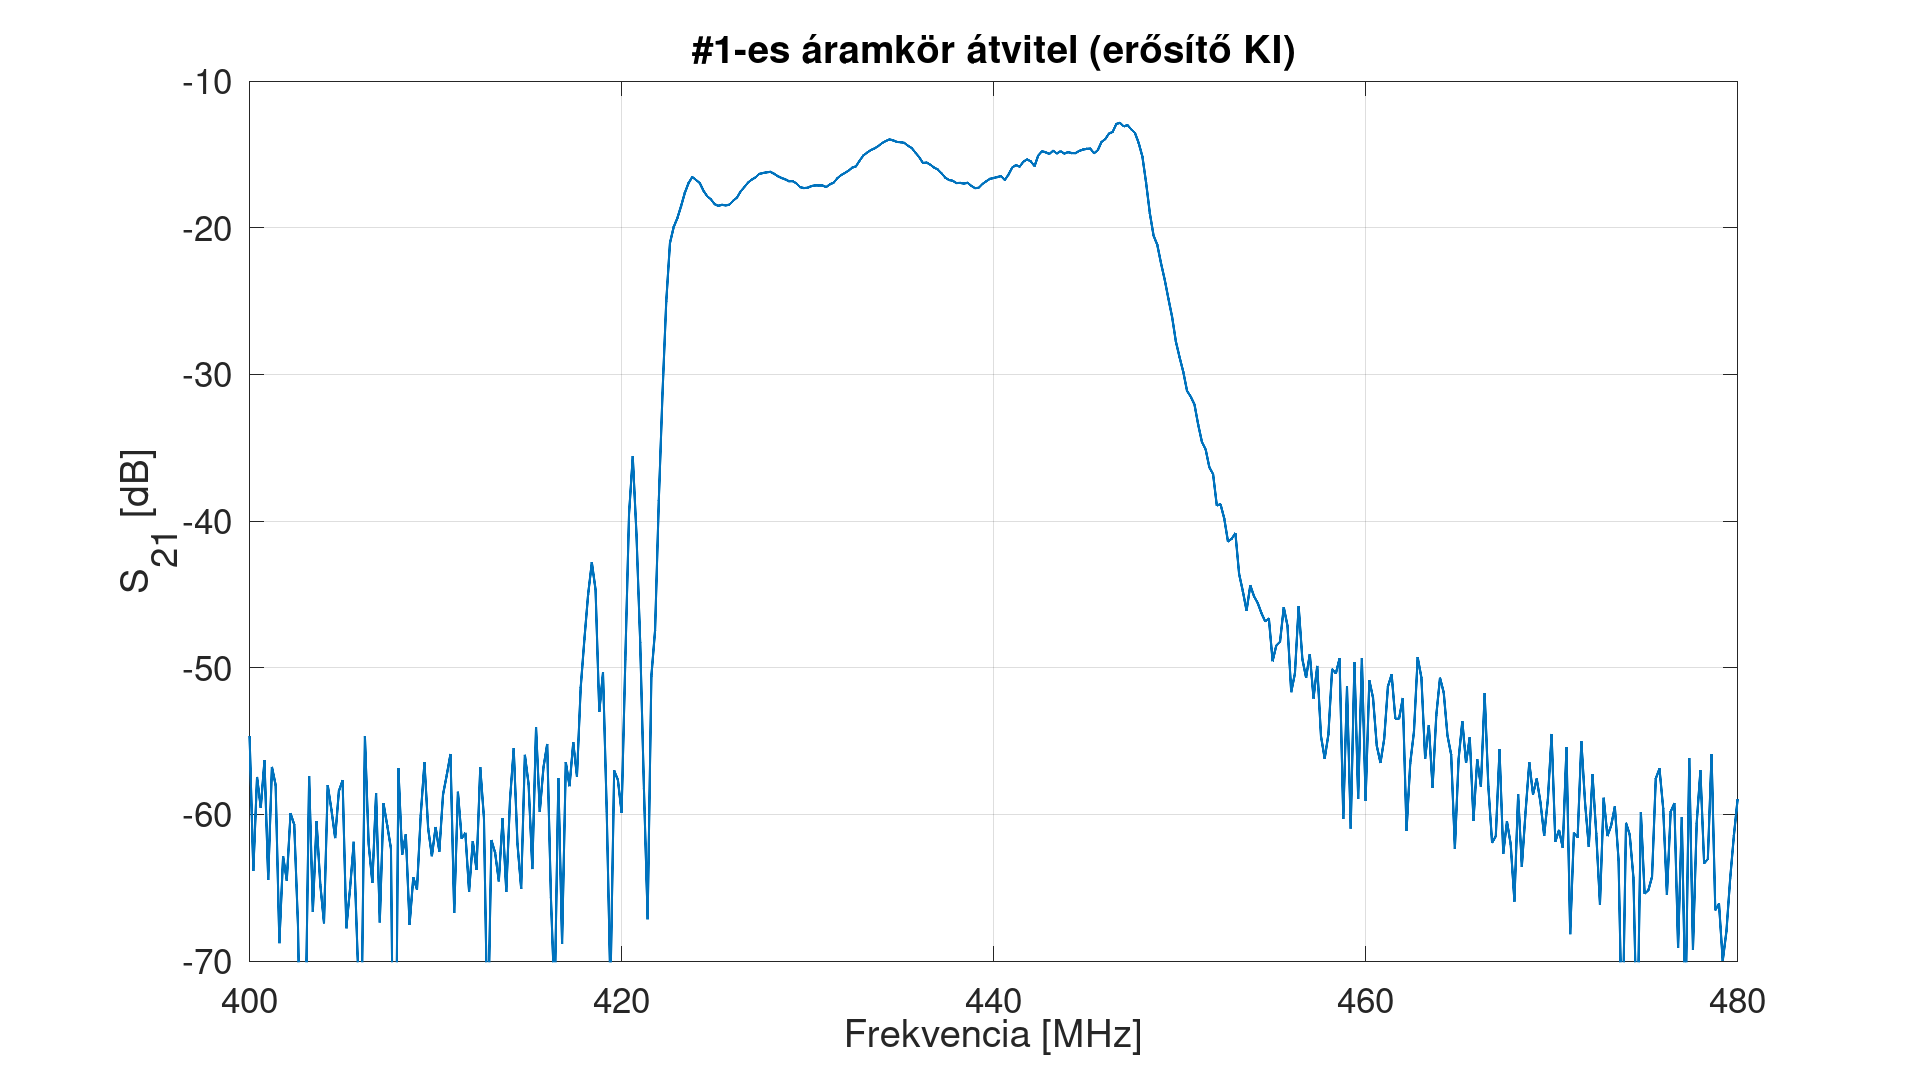
\includegraphics[keepaspectratio, width=\textwidth]{aramkor1_2.png}
	\caption{\#1-es erősítő 400\,MHz - 480\,MHz, erősítő KI}
	\label{fig:meres2}
\end{figure}

\begin{figure}[!ht]
	\centering
	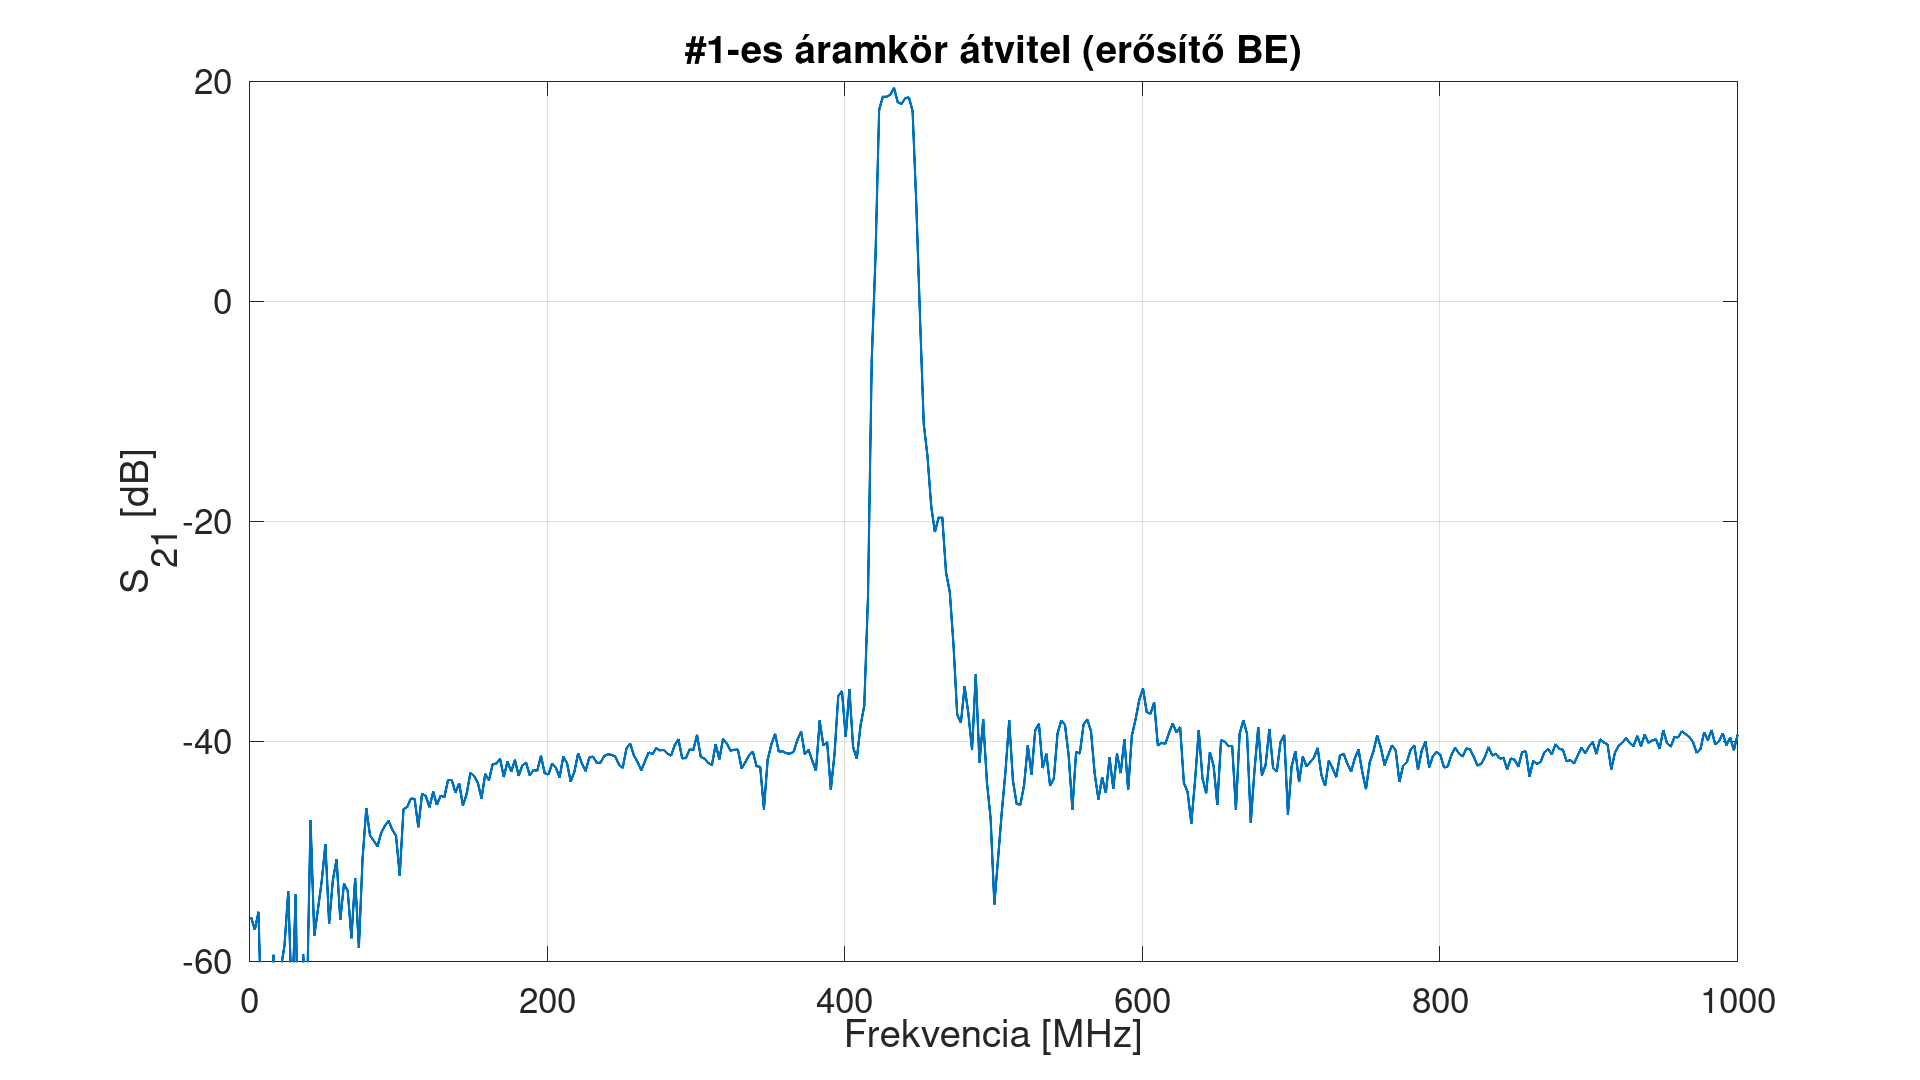
\includegraphics[keepaspectratio, width=\textwidth]{aramkor1_3.png}
	\caption{\#1-es erősítő 1\,MHz - 1\,GHz, erősítő BE}
	\label{fig:meres3}
\end{figure}

\begin{figure}[!ht]
	\centering
	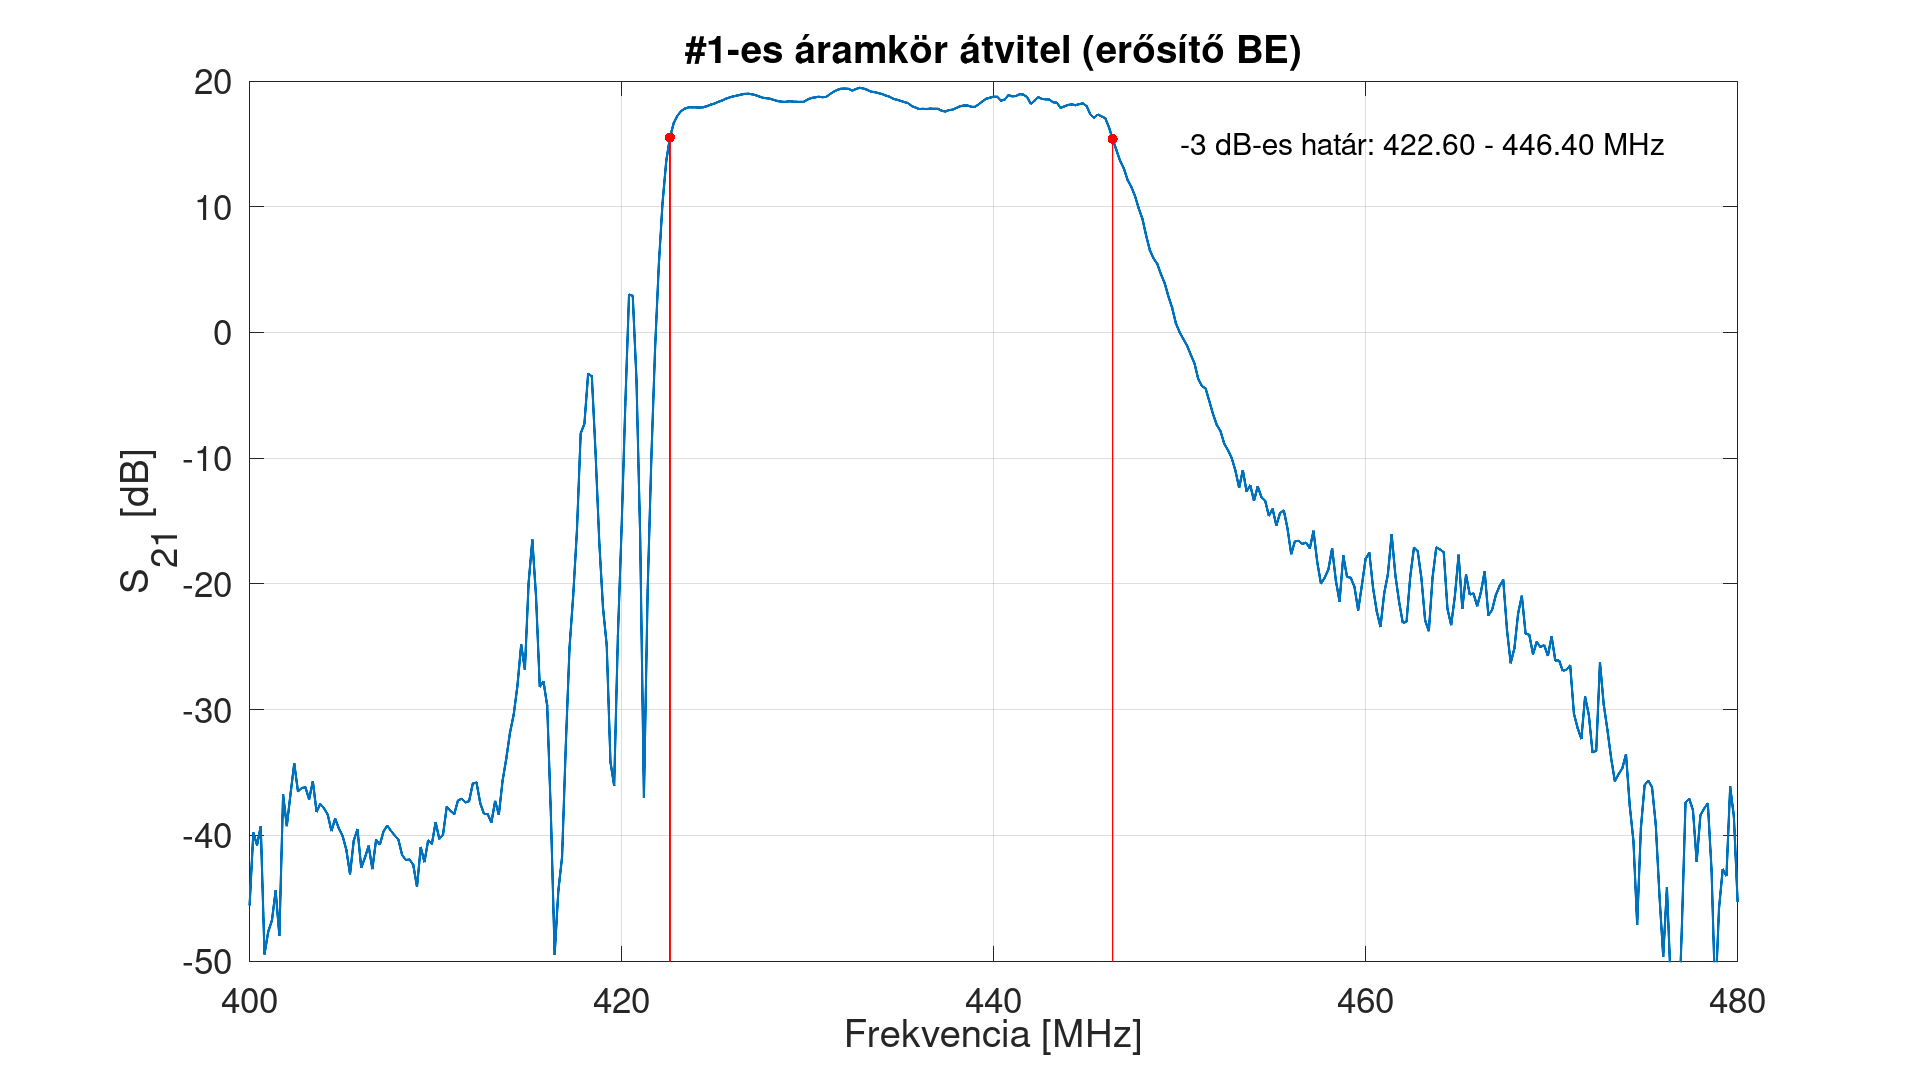
\includegraphics[keepaspectratio, width=\textwidth]{aramkor1_4.png}
	\caption{\#1-es erősítő 400\,MHz - 480\,MHz, erősítő BE}
	\label{fig:meres4}
\end{figure}



\begin{figure}[!ht]
	\centering
	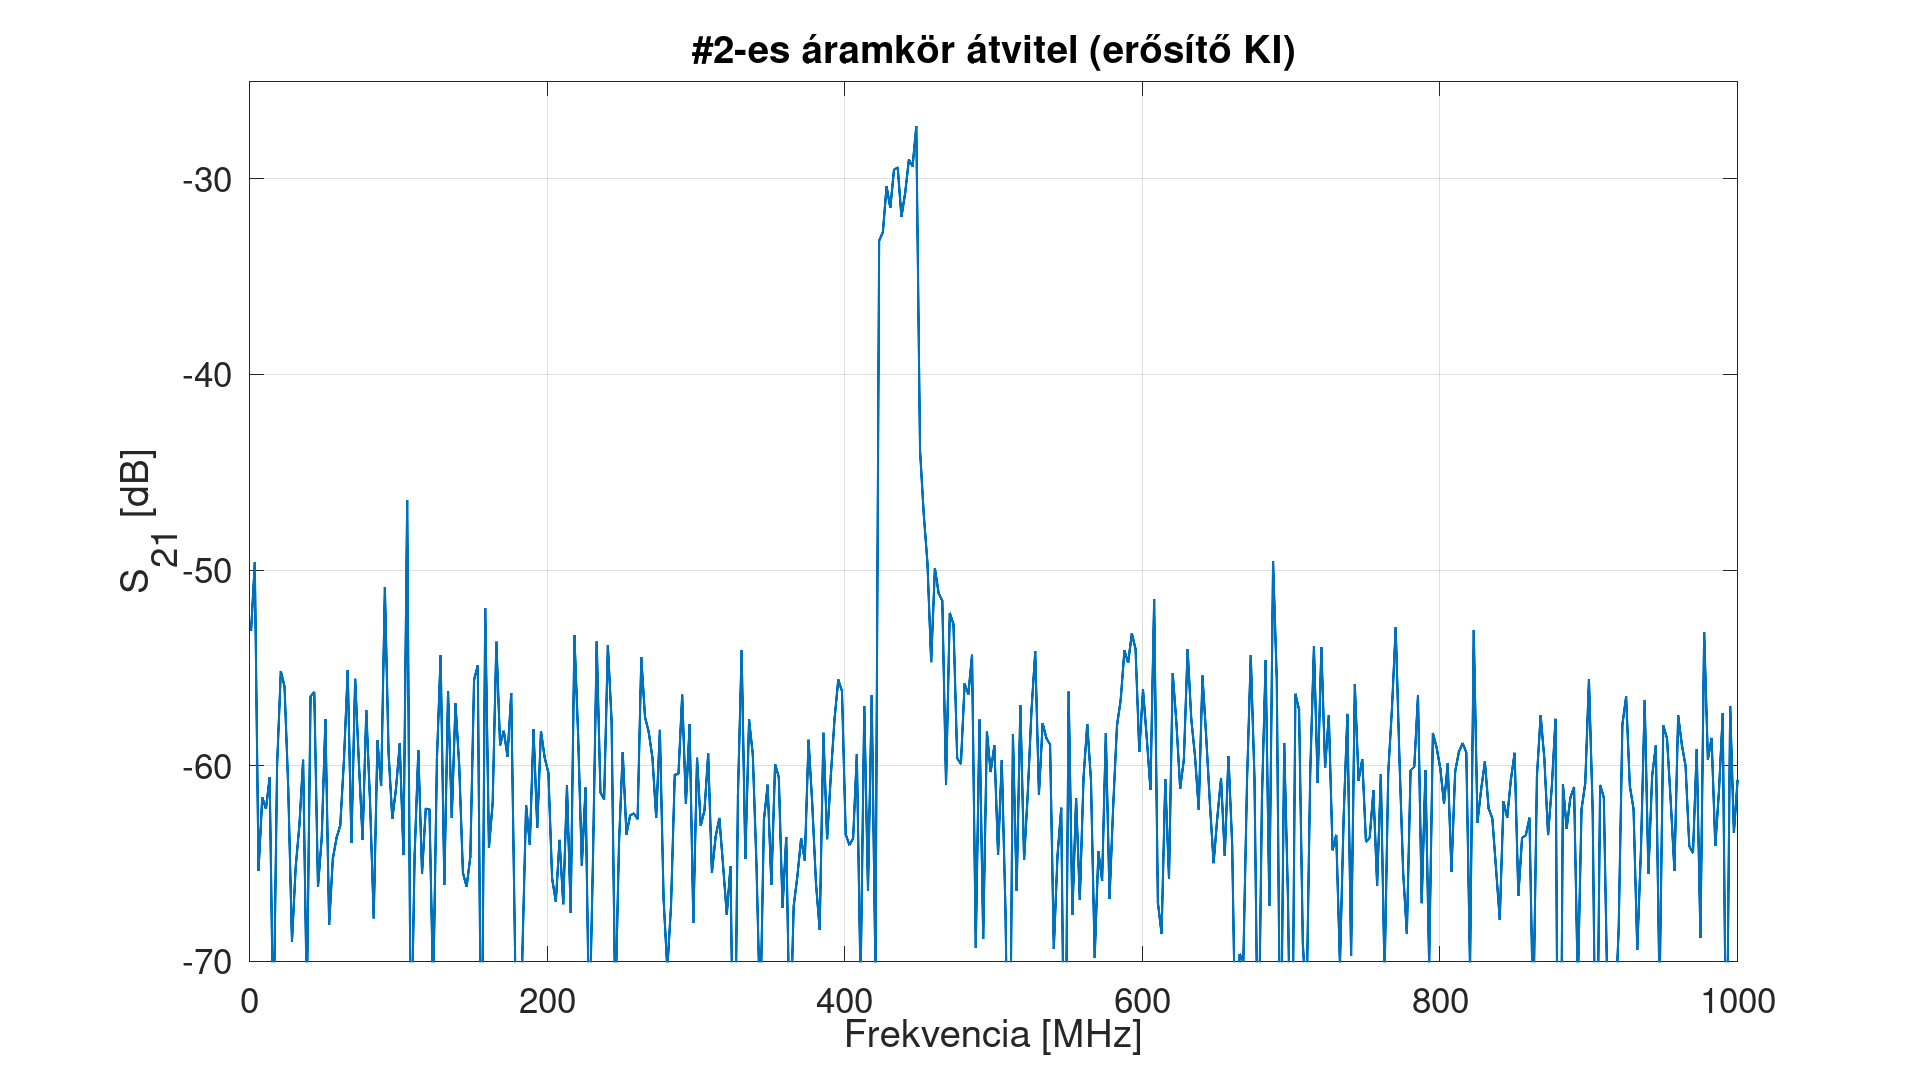
\includegraphics[keepaspectratio, width=\textwidth]{aramkor2_5.png}
	\caption{\#2-es erősítő 1\,MHz - 1\,GHz, erősítő KI}
	\label{fig:meres5}
\end{figure}

\begin{figure}[!ht]
	\centering
	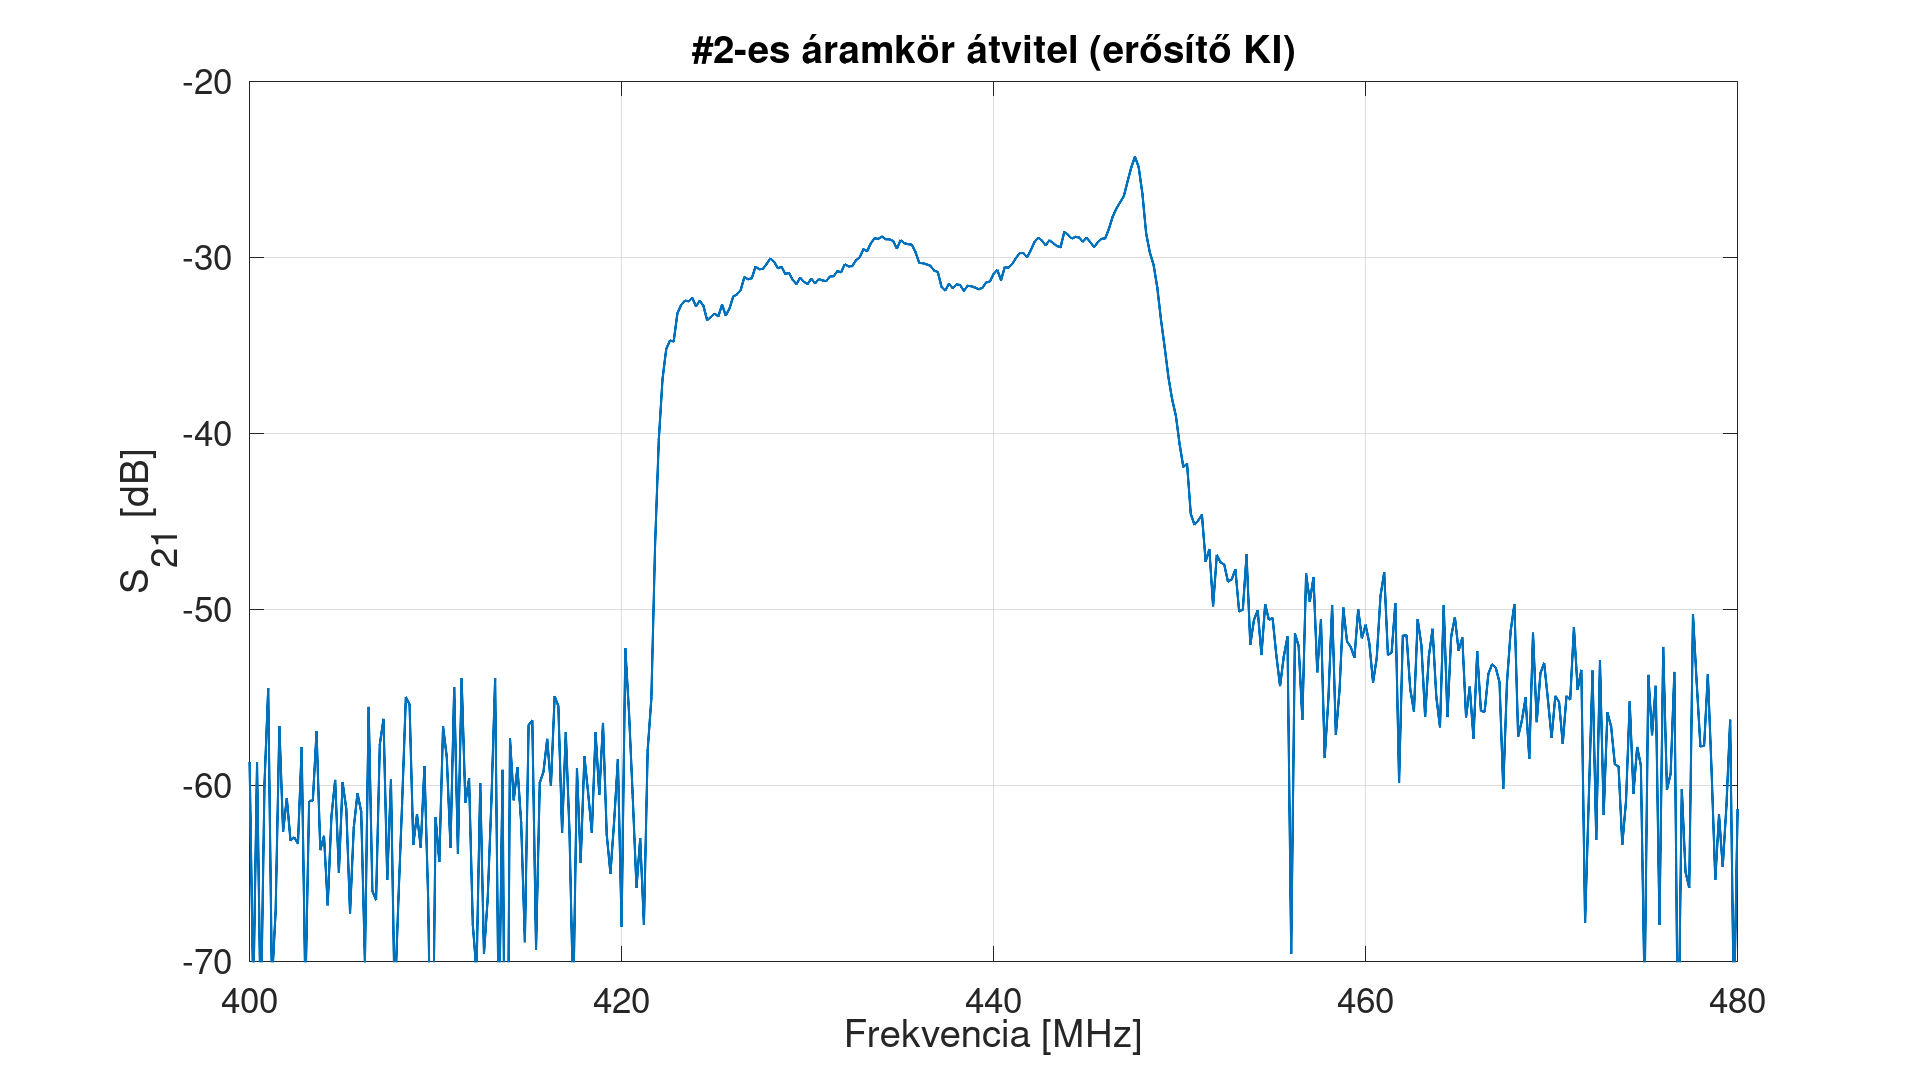
\includegraphics[keepaspectratio, width=\textwidth]{aramkor2_6.png}
	\caption{\#2-es erősítő 400\,MHz - 480\,MHz, erősítő KI}
	\label{fig:meres6}
\end{figure}

\begin{figure}[!ht]
	\centering
	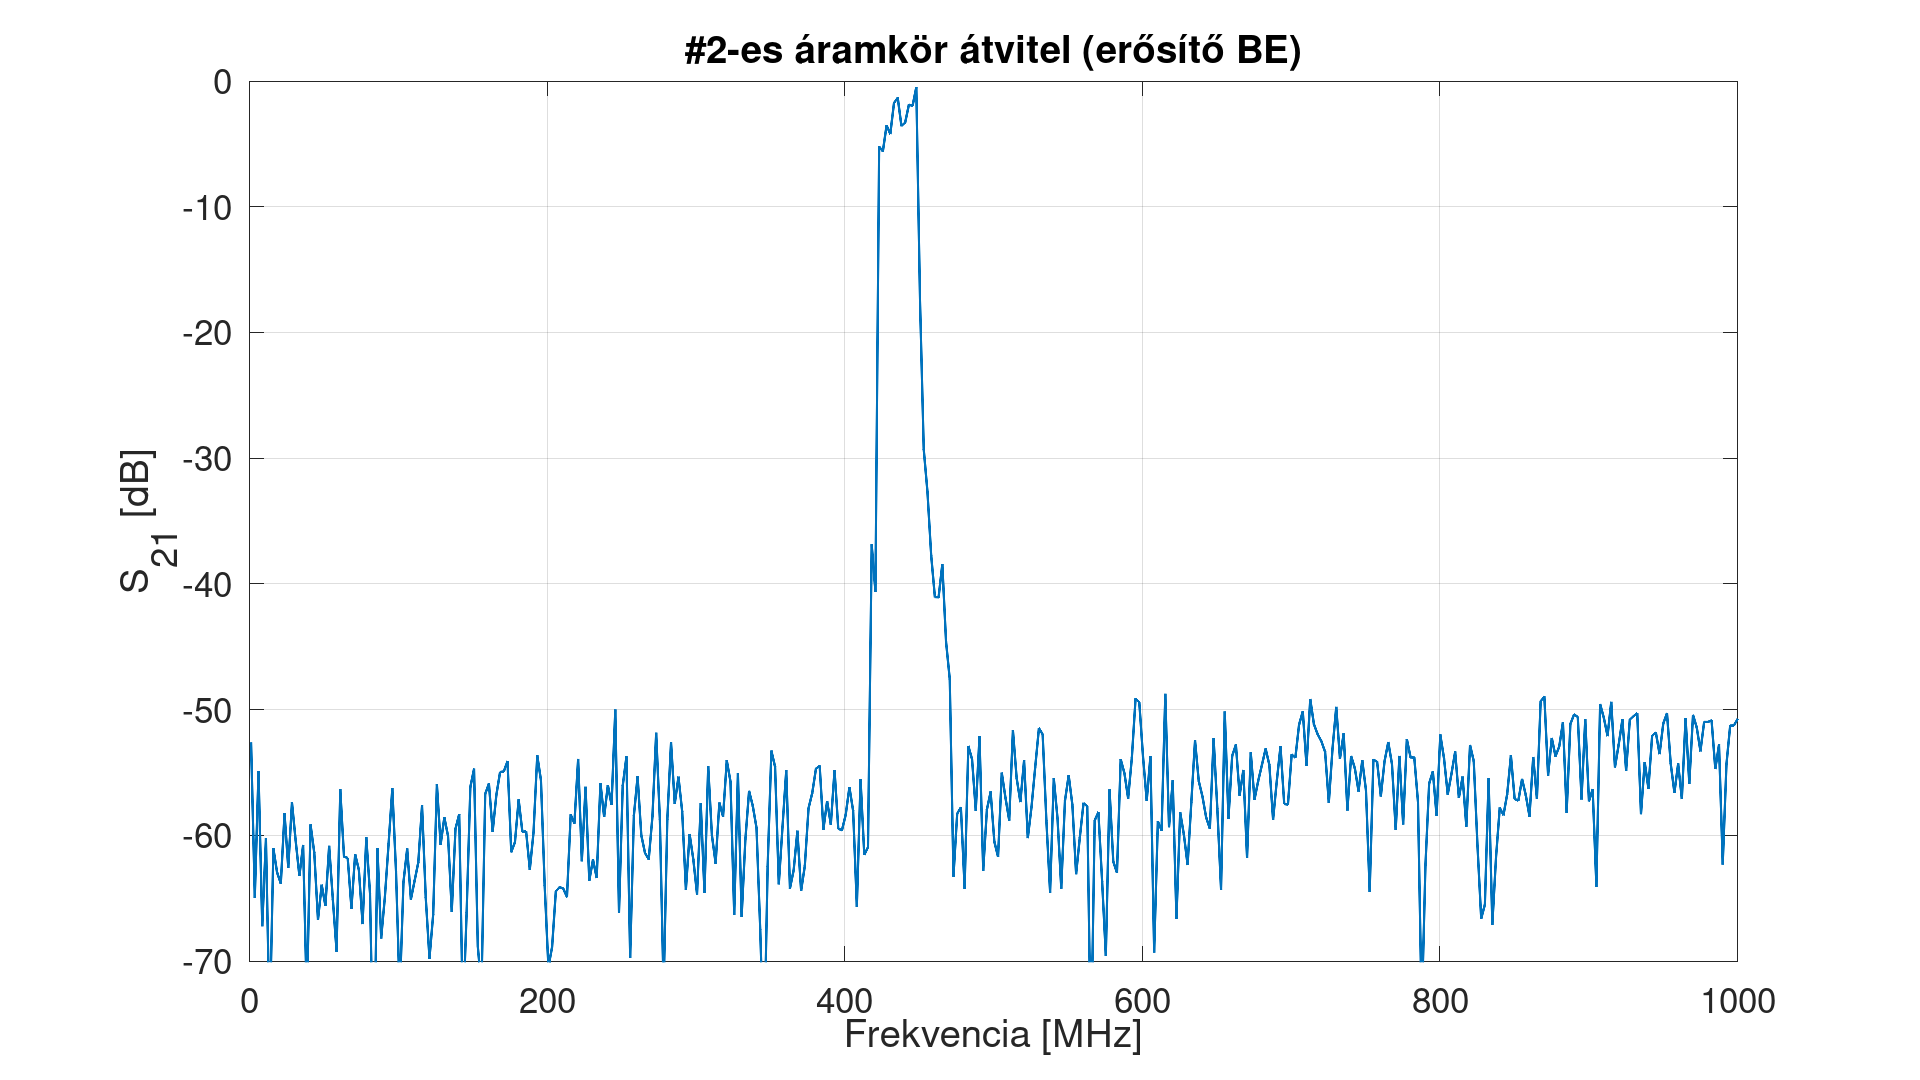
\includegraphics[keepaspectratio, width=\textwidth]{aramkor2_7.png}
	\caption{\#2-es erősítő 1\,MHz - 1\,GHz, erősítő BE}
	\label{fig:meres7}
\end{figure}

\begin{figure}[!ht]
	\centering
	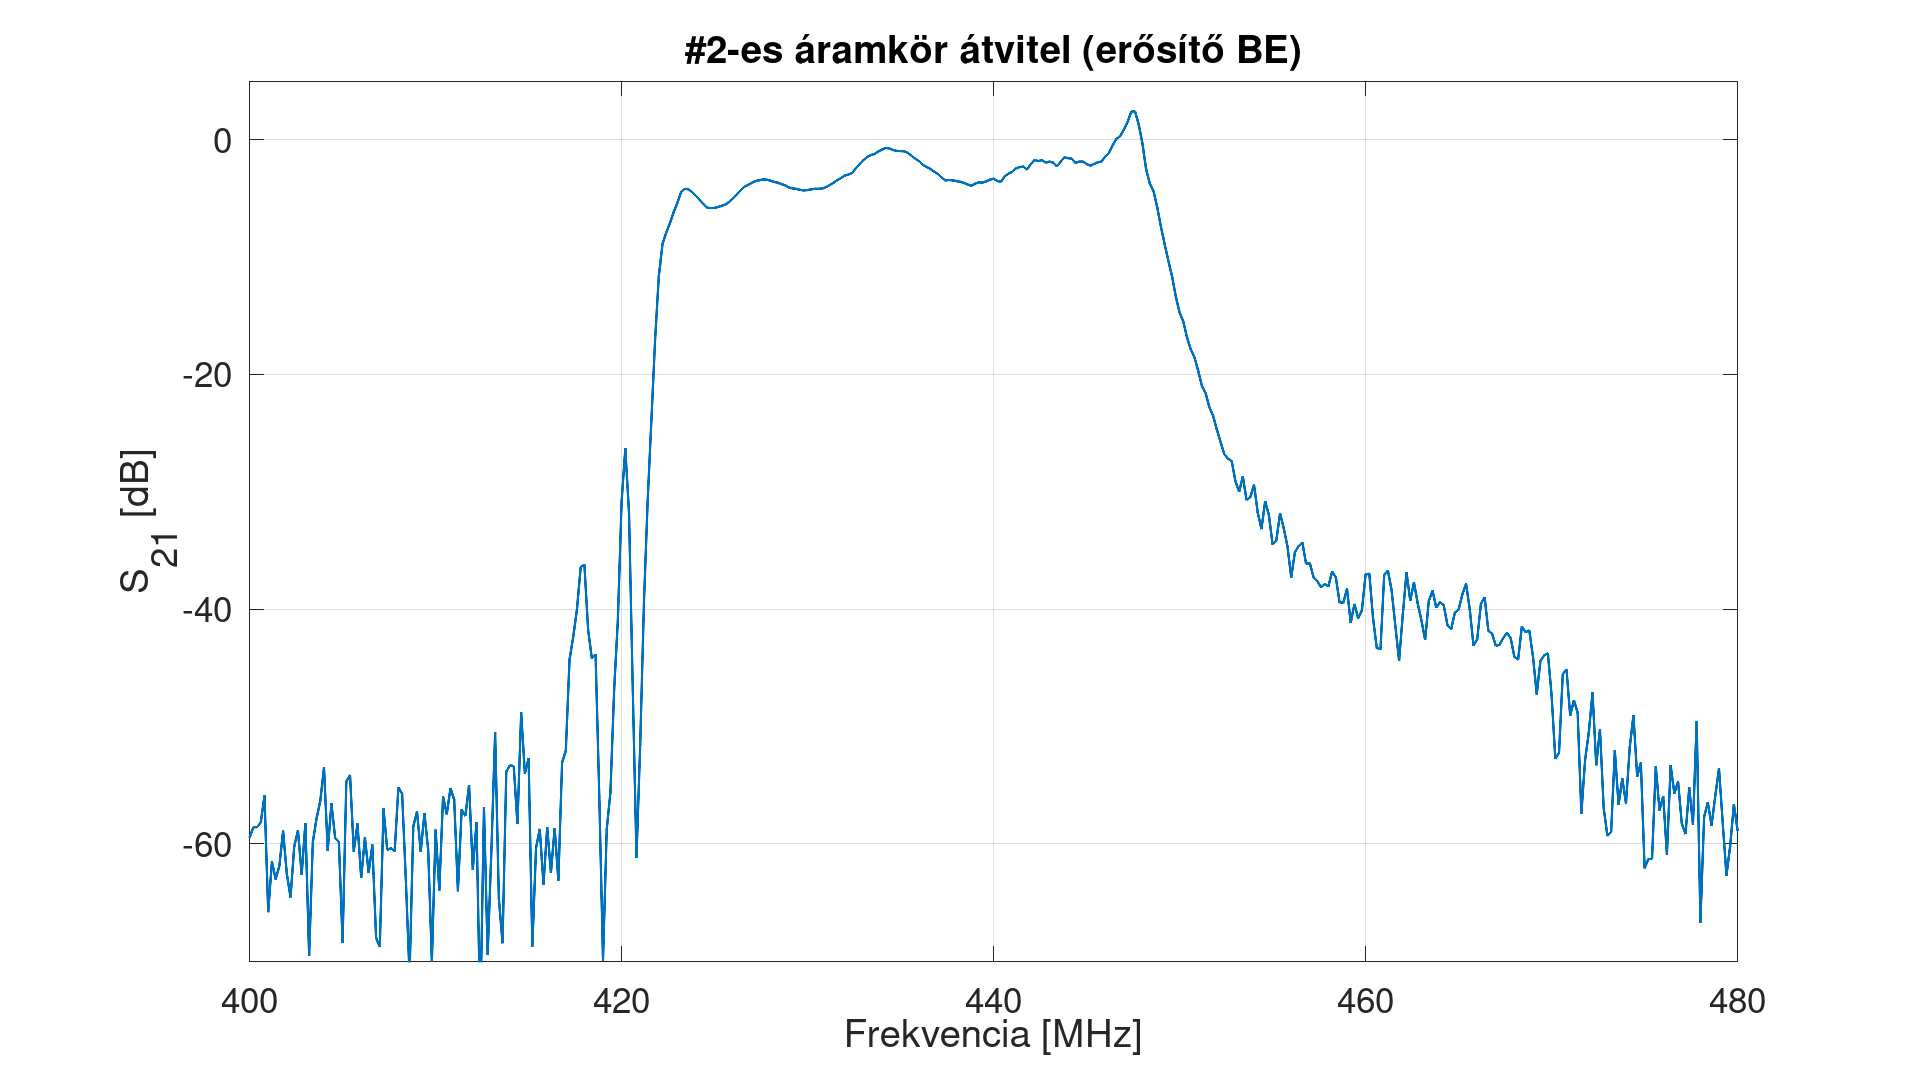
\includegraphics[keepaspectratio, width=\textwidth]{aramkor2_8.png}
	\caption{\#2-es erősítő 400\,MHz - 480\,MHz, erősítő BE}
	\label{fig:meres8}
\end{figure}

\begin{figure}[!ht]
	\centering
	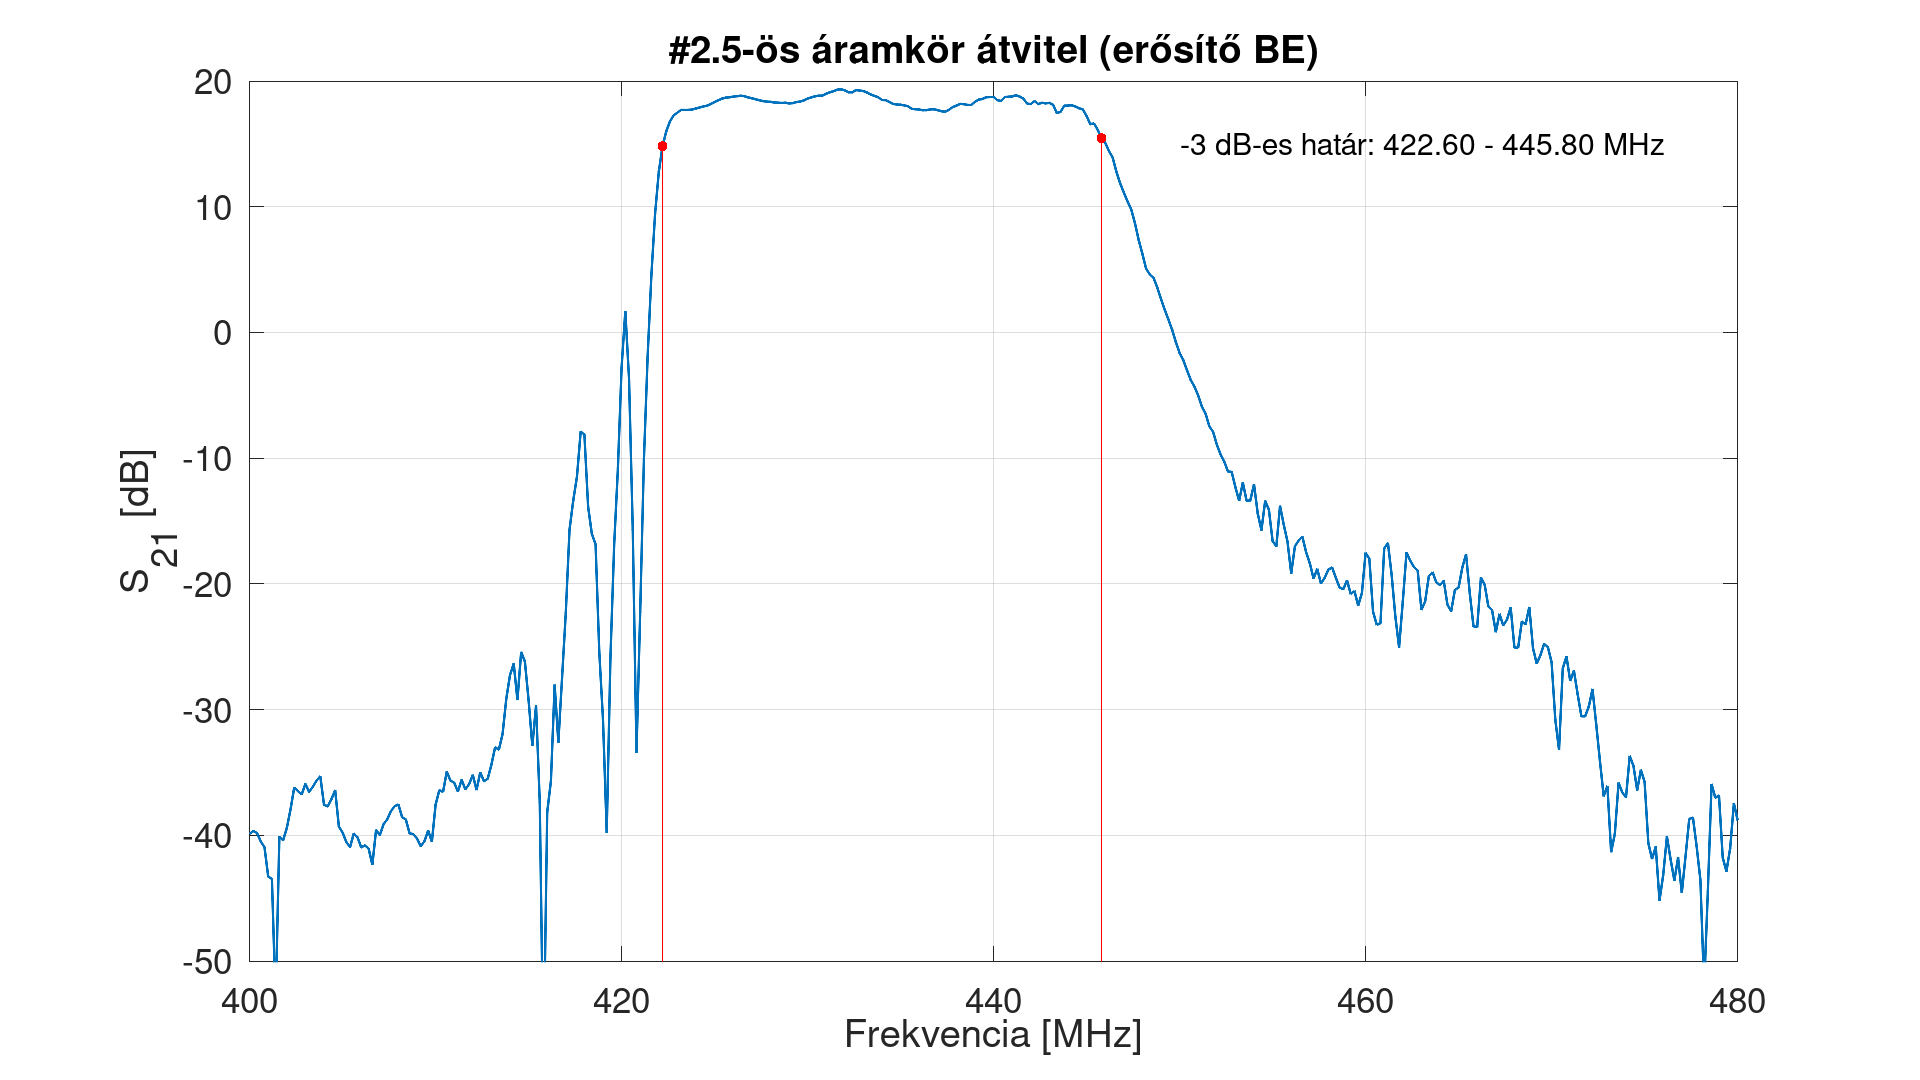
\includegraphics[keepaspectratio, width=\textwidth]{aramkor2_14.png}
	\caption{\#2.5-ös erősítő 400\,MHz - 480\,MHz, erősítő BE}
	\label{fig:meres14}
\end{figure}



\begin{figure}[!ht]
	\centering
	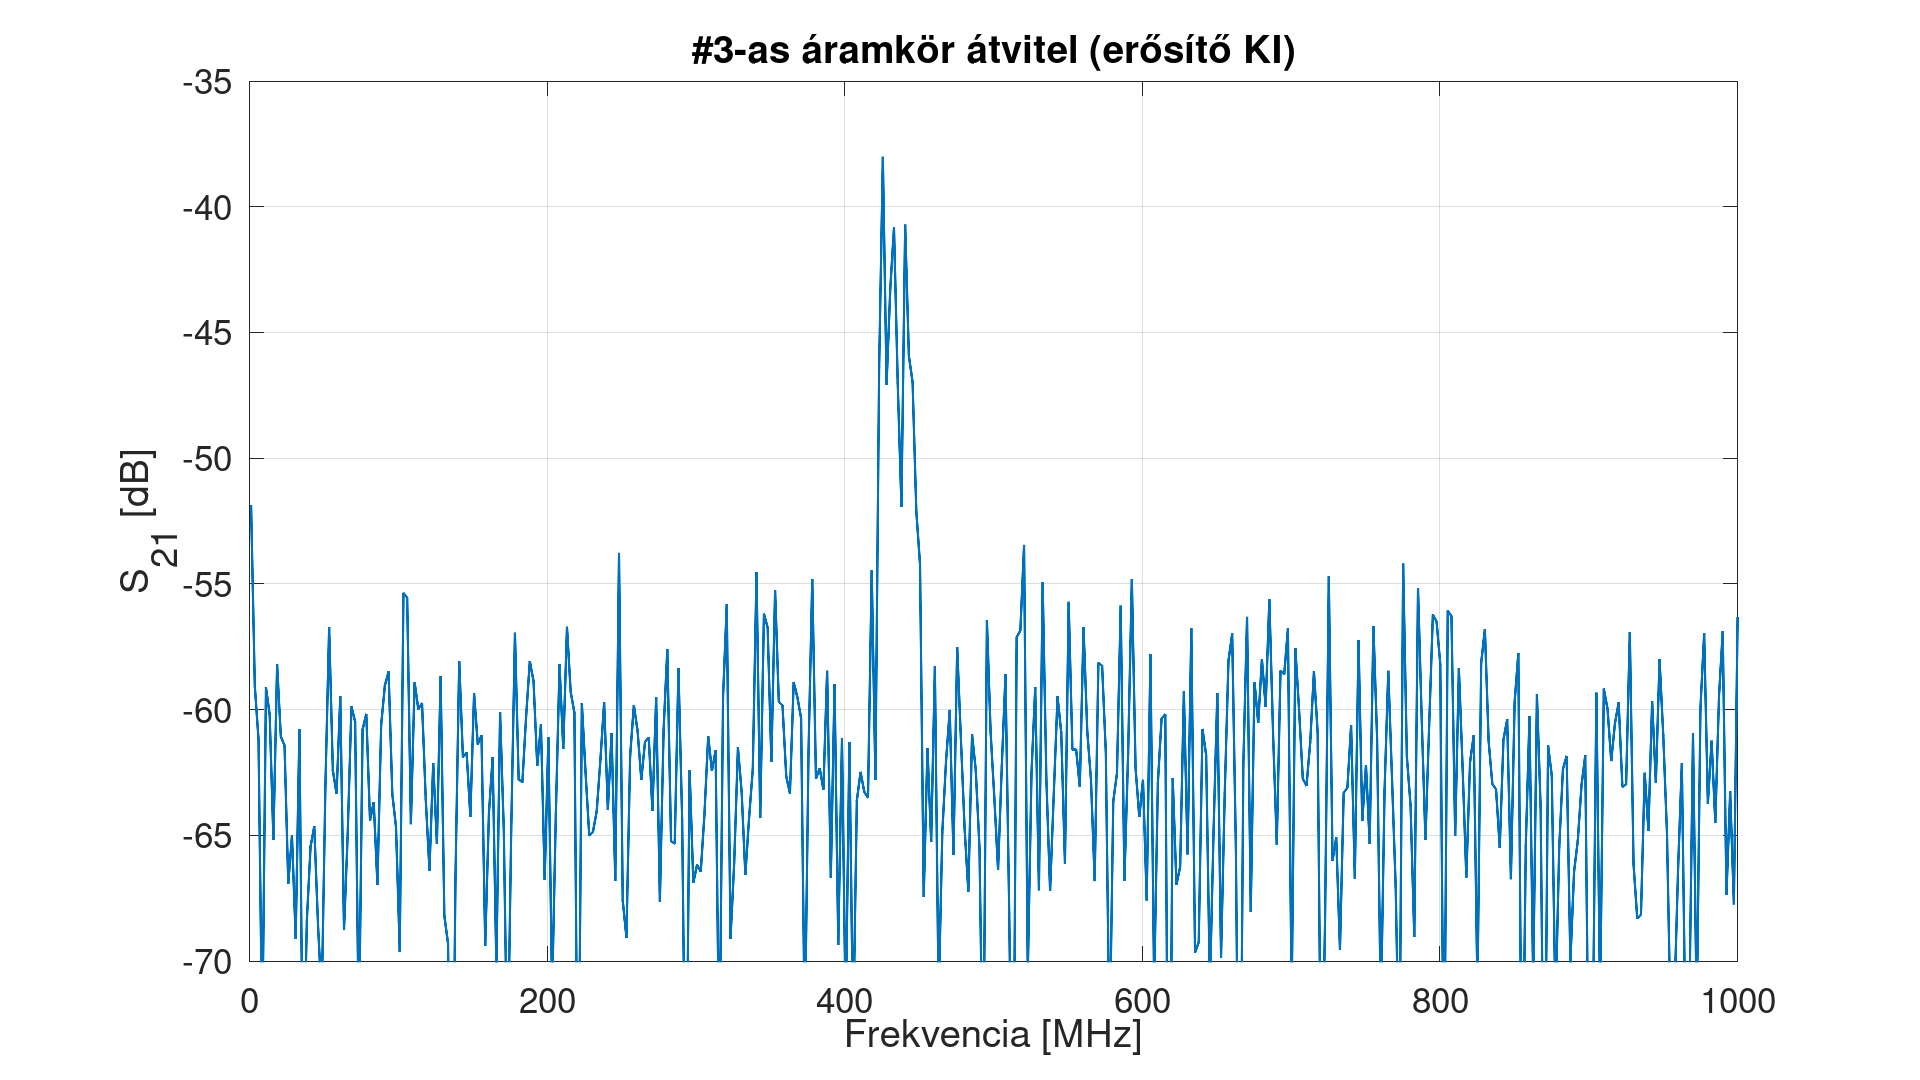
\includegraphics[keepaspectratio, width=\textwidth]{aramkor3_9.png}
	\caption{\#3-as erősítő 1\,MHz - 1\,GHz, erősítő KI}
	\label{fig:meres9}
\end{figure}

\begin{figure}[!ht]
	\centering
	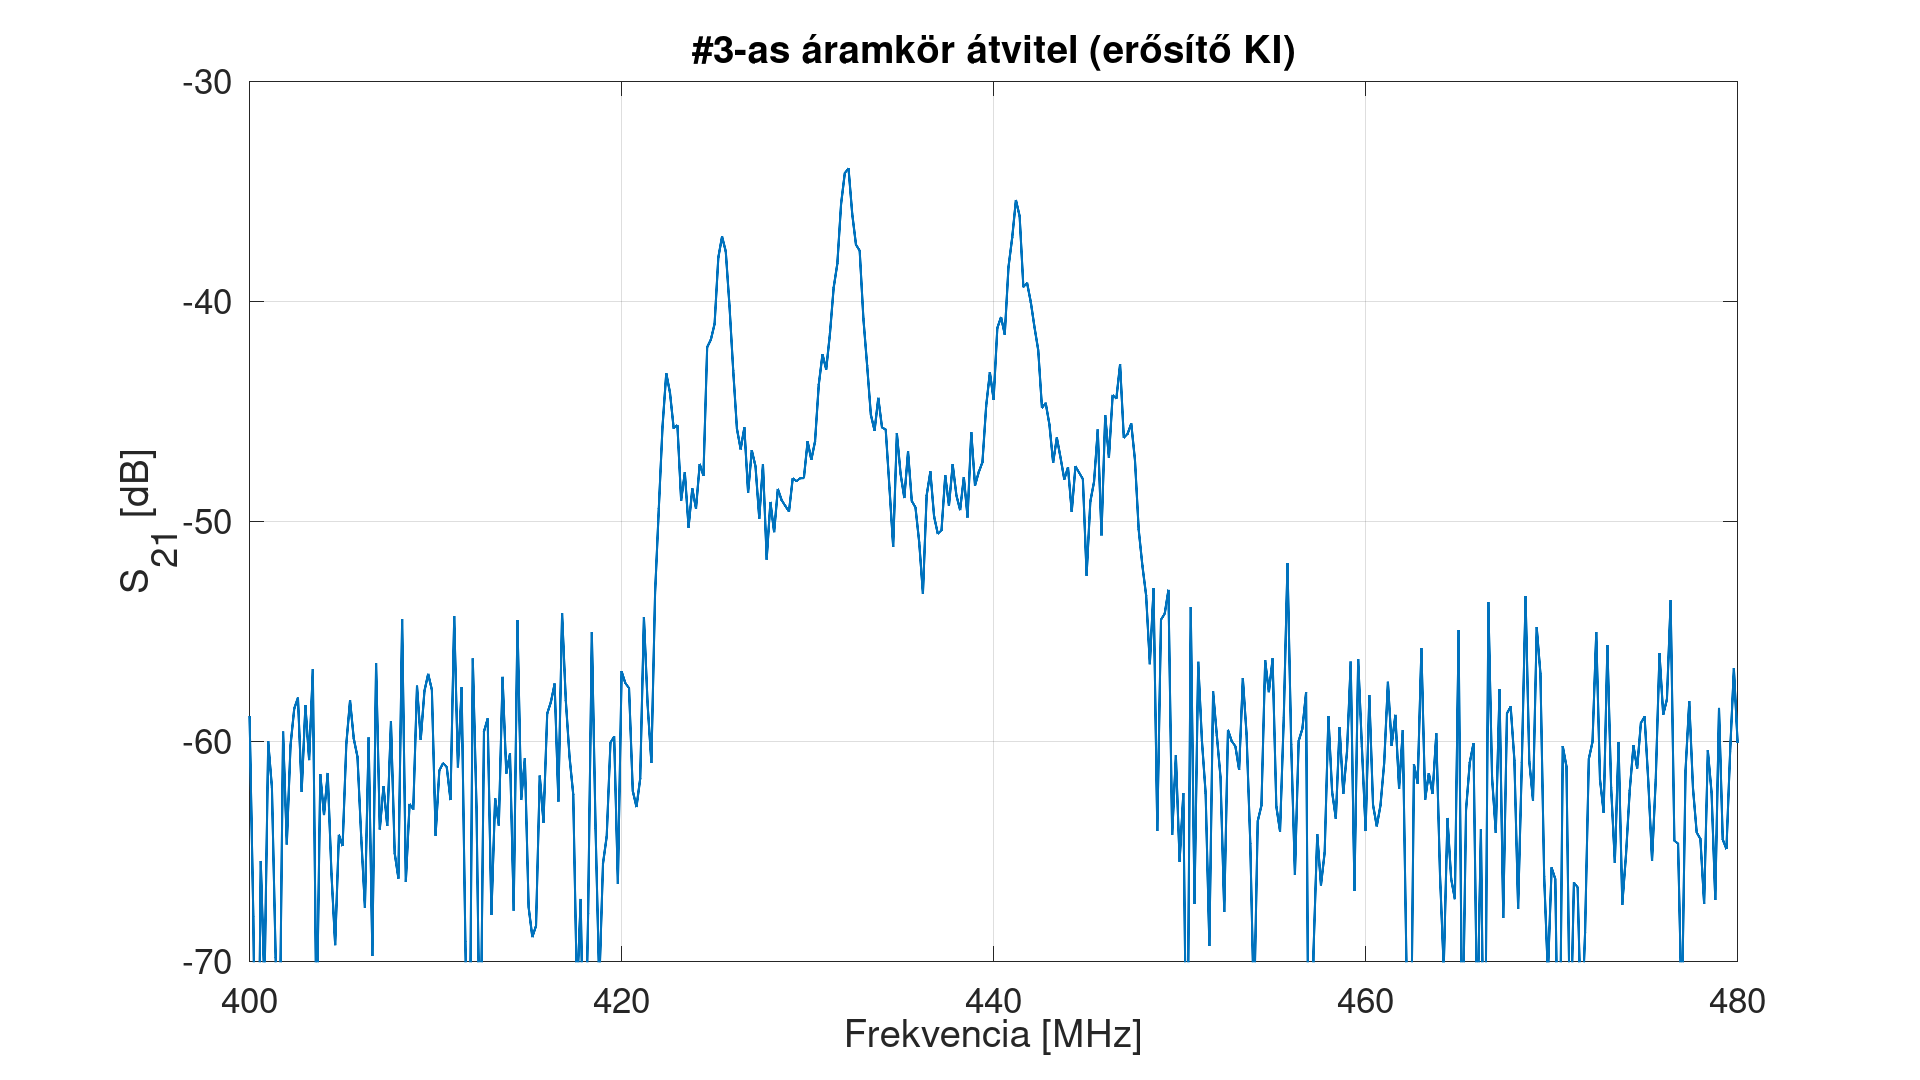
\includegraphics[keepaspectratio, width=\textwidth]{aramkor3_10.png}
	\caption{\#3-as erősítő 400\,MHz - 480\,MHz, erősítő KI}
	\label{fig:meres10}
\end{figure}

\begin{figure}[!ht]
	\centering
	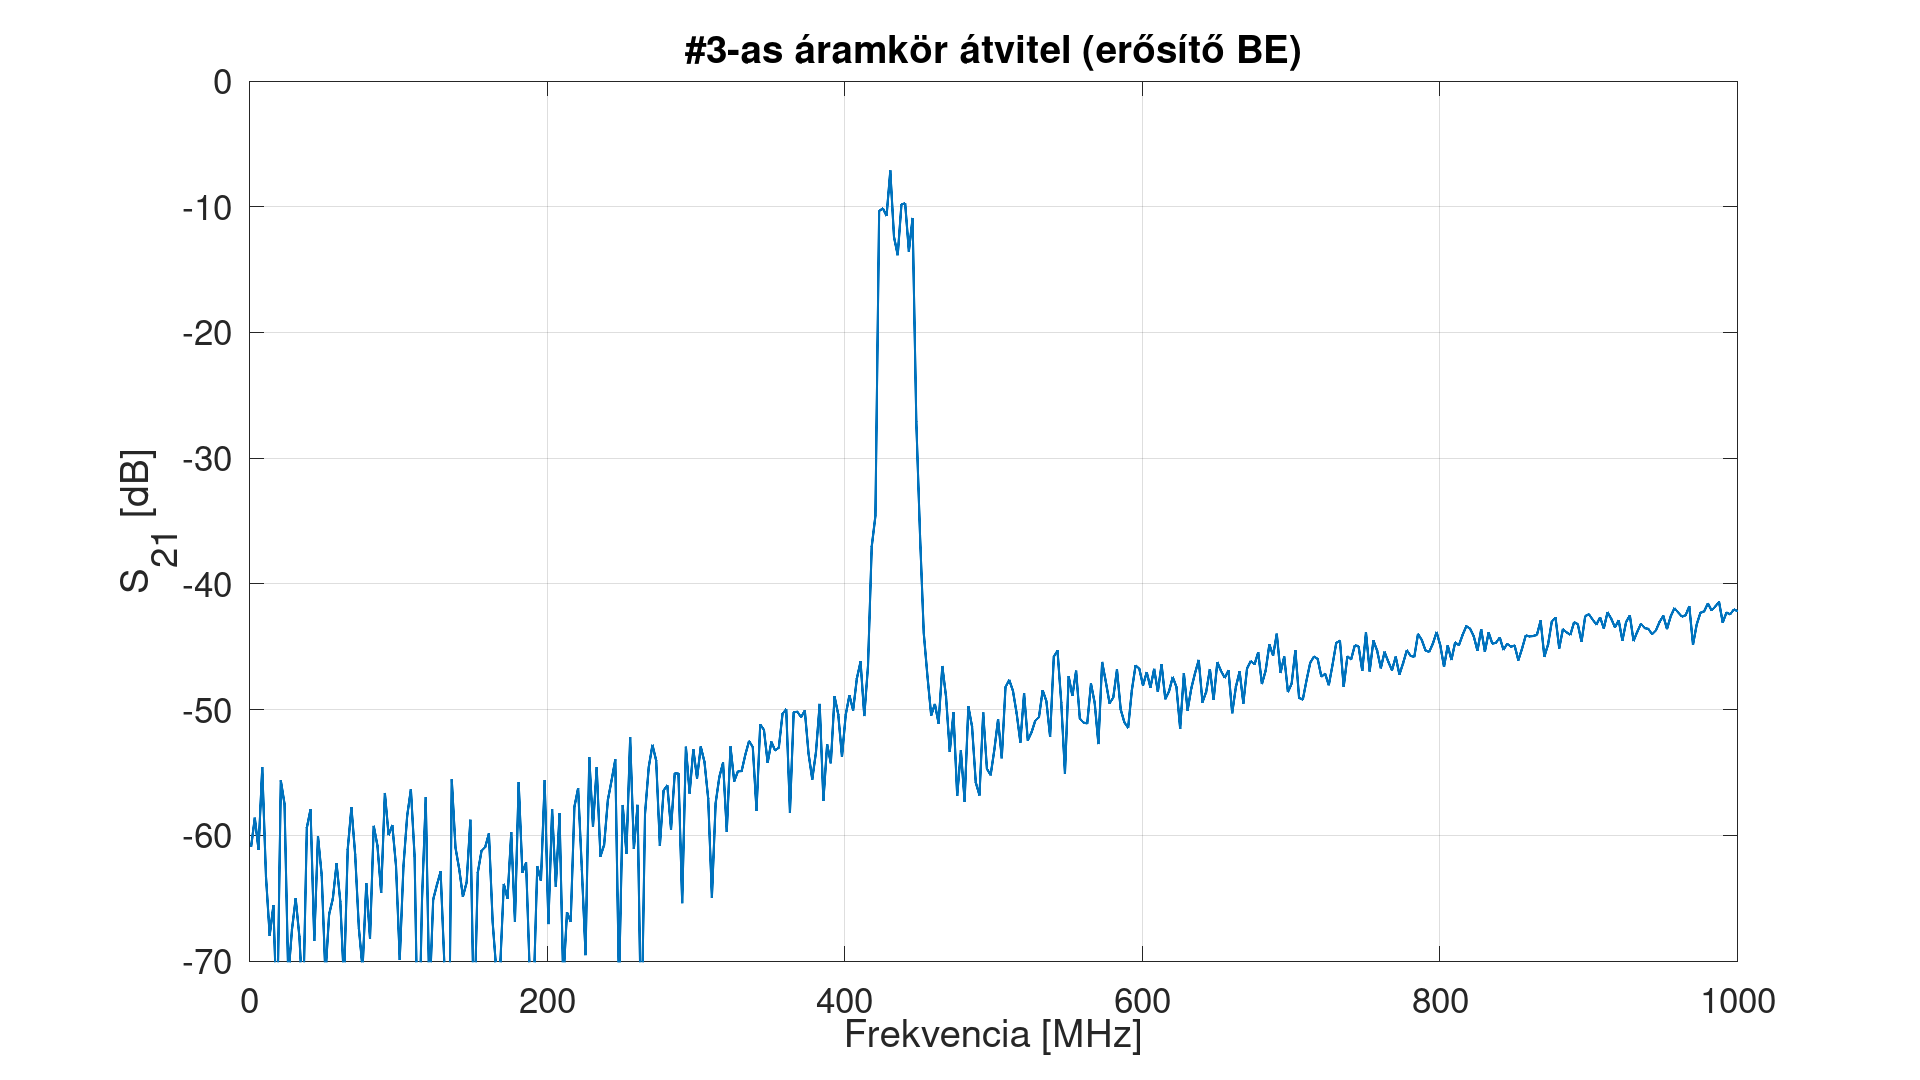
\includegraphics[keepaspectratio, width=\textwidth]{aramkor3_11.png}
	\caption{\#3-as erősítő 1\,MHz - 1\,GHz, erősítő BE}
	\label{fig:meres11}
\end{figure}

\begin{figure}[!ht]
	\centering
	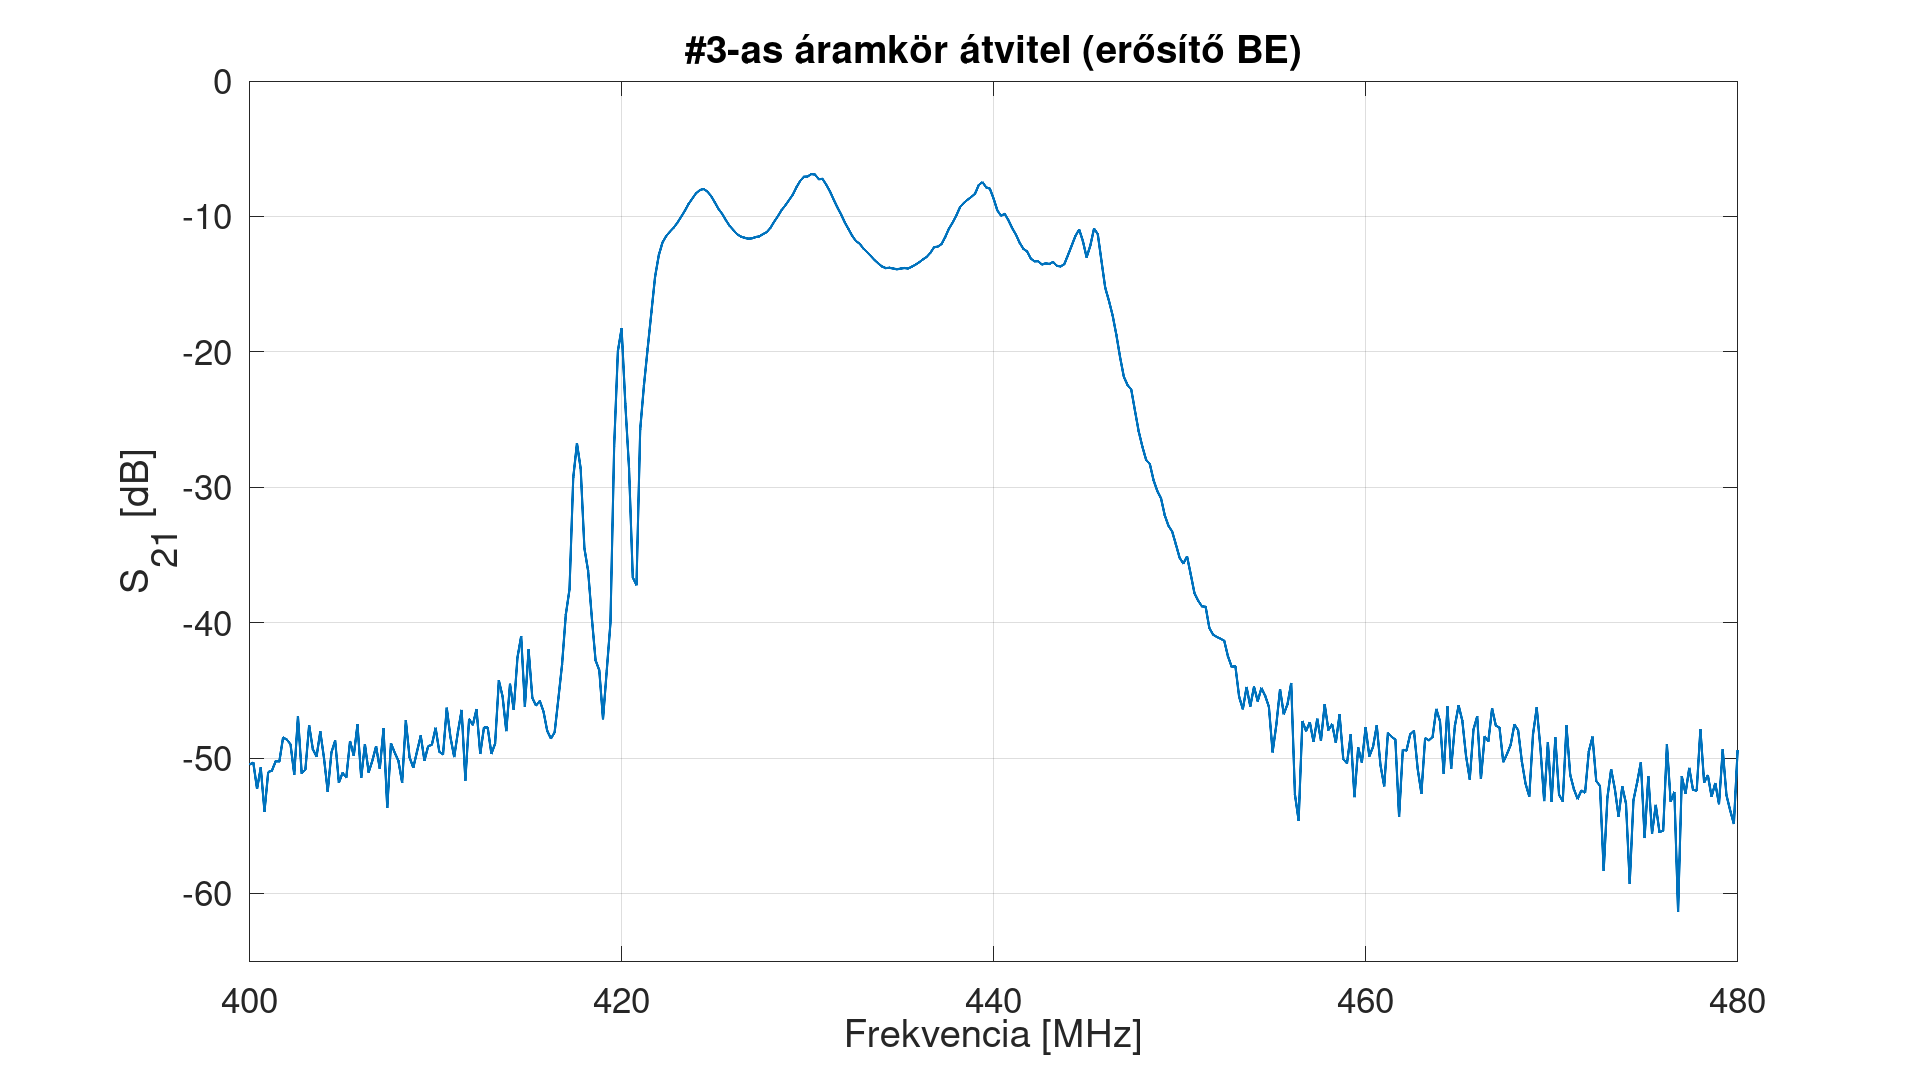
\includegraphics[keepaspectratio, width=\textwidth]{aramkor3_12.png}
	\caption{\#3-as erősítő 400\,MHz - 480\,MHz, erősítő BE}
	\label{fig:meres12}
\end{figure}

\newpage
